\documentclass[12pt]{article}
\usepackage{graphicx}
\usepackage{amsmath}
\usepackage{mathtools}
\usepackage{gensymb}

\newcommand{\mydet}[1]{\ensuremath{\begin{vmatrix}#1\end{vmatrix}}}
\providecommand{\brak}[1]{\ensuremath{\left(#1\right)}}
\providecommand{\norm}[1]{\left\lVert#1\right\rVert}
\newcommand{\solution}{\noindent \textbf{Solution: }}
\newcommand{\myvec}[1]{\ensuremath{\begin{pmatrix}#1\end{pmatrix}}}
\let\vec\mathbf

\begin{document}
\begin{center}
\textbf\large{CHAPTER-10 \\ STRAIGHT LINES}
\end{center}
\section*{Excercise 10.3}

Q3. Reduce the following equations into normal form. Find their perpendicular distances from the origin and angle between perpendicular and the positive $x$-axis.
\begin{enumerate}
	\item $x-\sqrt{3}y+8=0$ 
	\item $y-2=0$
	\item $x-y=4$
\end{enumerate}
\solution
\begin{enumerate}
\item From the given equation:
	\begin{align}
		\vec{m}&=\frac{1}{\sqrt{3}}\\
		c&=\frac{8}{\sqrt{3}}
	\end{align}
        The directional vector is given by:
	\begin{align}
		\vec{m}&=\myvec{1\\\frac{1}{\sqrt{3}}\\}
	\end{align}
	The normal vector is given by:
		\begin{align}
	\vec{n}&=\myvec{-\frac{1}{\sqrt{3}}\\1\\}\\
	\vec{n}^\top&=\myvec{-\frac{1}{\sqrt{3}} & 1}\\
			\norm{\vec{n}}&=\sqrt{\vec{n}^\top.\vec{n}}\\
			&=\frac{2}{\sqrt{3}}
			\end{align}
	Slope of normal is given by:
		\begin{align}
			\tan\theta=-\frac{1}{\vec{m}}=-\frac{1}{\frac{1}{\sqrt{3}}}=-\sqrt{3}\\
			\theta=120^\circ
		\end{align}
	The perpendicular distance from the origin to the line is given by:
		\begin{align}
			d=\frac{|c|}{\norm{\vec{n}}}=\frac{8}{2}\\
			=4
		\end{align}
\begin{figure}[!h]
	\begin{center} 
	    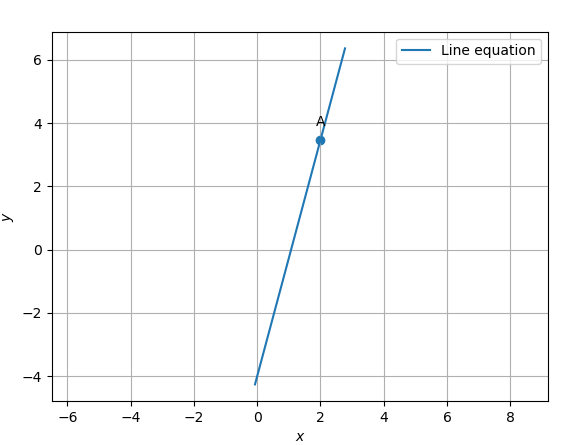
\includegraphics[width=\columnwidth]{./figs/line.png}
	\end{center}
\caption{}
\label{fig:Fig}
\end{figure}
	

\item From the given equation:
         \begin{align}                                                                                                 \vec{m}&=0\\                                                                        			c&=2
         \end{align}                                                                                          The directional vector is given by:
          \begin{align}
                  \vec{m}&=\myvec{1\\0\\}
          \end{align}
          The normal vector is given by:
                  \begin{align}
         \vec{n}&=\myvec{0\\1\\}\\
          \vec{n}^\top&=\myvec{0 & 1}\\
                       \norm{\vec{n}}&=\sqrt{\vec{n}^\top.\vec{n}}\\
                          &=1
                          \end{align}
          Slope of normal is given by:
		\begin{align}                                                                                                 \tan\theta=-\frac{1}{\vec{m}}=-\frac{1}{0}=\infty\\                             \theta=90^\circ
                \end{align}                                                                                 The perpendicular distance from the origin to the line is given by:                                          \begin{align}
			d=\frac{|c|}{\norm{\vec{n}}}=\frac{2}{1}\\                                                              =2
                  \end{align}
                  
                  \begin{figure}[!h]
	\begin{center} 
	    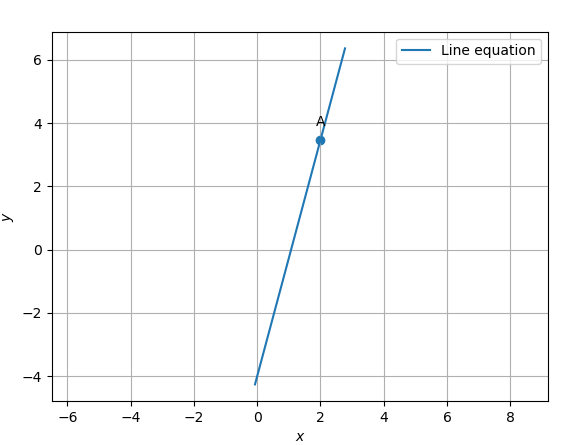
\includegraphics[width=\columnwidth]{./figs/line.png}
	\end{center}
\caption{}
\label{fig:Fig}
\end{figure}
	
	
\item From the given equation:
         \begin{align}                                                                                                 \vec{m}&=1\\                                                                        			c&=-4
         \end{align}                                                                                          The directional vector is given by:
          \begin{align}
                  \vec{m}&=\myvec{1\\1\\}
          \end{align}
          The normal vector is given by:
                  \begin{align}
         \vec{n}&=\myvec{-1\\1\\}\\
          \vec{n}^\top&=\myvec{-1 & 1}\\
                       \norm{\vec{n}}&=\sqrt{\vec{n}^\top.\vec{n}}\\
                          &=\sqrt{2}
                          \end{align}
          Slope of normal is given by:
		\begin{align}                                                                                                 \tan\theta=-\frac{1}{\vec{m}}=-\frac{1}{1}=-1\\                             \theta=315^\circ
                \end{align}                                                                                 The perpendicular distance from the origin to the line is given by:                                          \begin{align}
			d=\frac{|c|}{\norm{\vec{n}}}=\frac{4}{\sqrt{2}}\\=2\sqrt{2}                                                      
                  \end{align}

\begin{figure}[!h]
	\begin{center} 
	    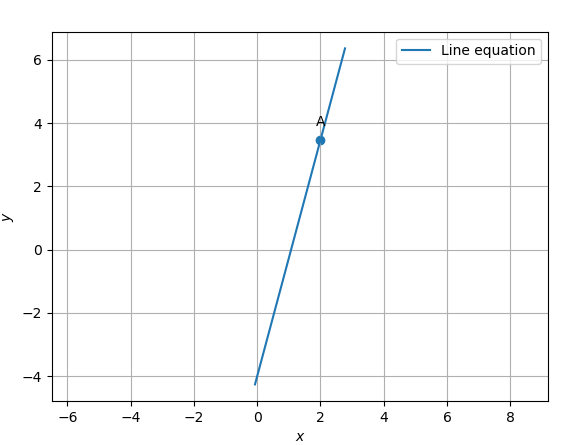
\includegraphics[width=\columnwidth]{./figs/line.png}
	\end{center}
\caption{}
\label{fig:Fig}
\end{figure}
\end{enumerate}
\end{document}
